\section{Implementation}\label{sec:implementation}

\subsection{General sequential version (\textit{seq})}\label{ssec:seq-implementation}
We implement the Leapfrog Triejoin~\cite{leapfrog} as our general sequential version of a WCOJ.
However, instead of using B-Trees as a backing data structure, we use sorted arrays and a binary
search, which has been described in~\cite{myria-detailed} and is called
Tributary join in their paper.
Our Leapfrog Triejoin is implemented in three components which we explain in order below: \textit{LeapfrogJoin}, \textit{ArrayTrieIterable} and
\textit{LeapfrogTriejoin}.

The Leapfrog join is a variant of the sort-merge join for unary relationships, originally described in~\cite{leapfrog1,leapfrog2}. % TODO see LFTJ paper 4 and 7
To join $k$ unary relations $A_1(x)$, $A_2(x)$, \dots, $A_k(x)$ it takes one iterator per input relations and offers an iterator
interface that yields the intersection of all relations.
It requires that it's input iterators offer a \textit{key} method in $\mathcal{O}(1)$, a \textit{next} method and
a \textit{leastUpperBound(key: Int)} both in $\mathcal{O} (\log n)$ ($n$ defined as the size of the input relationship).
\textit{leastUpperBound} moves the iterator to the first position of the sought \textit{key} or the first position of the
next higher value.
An idiotmatic implementation of a Leapfrog join is shown in~\cref{lst:leapfrog-join}, for the optimized implementation see
\texttt{leapfrogTriejoin.LeapfrogJoin} in our repository.  % CODEREF

\begin{listing}[H]
    \inputminted[linenos=true]{scala}{code/LeapfrogJoin.scala}
    \caption{Leapfrog join.}
    \label{lst:leapfrog-join}
\end{listing}

To support j-arity relations, $A(a_1, a_2, \dots, a_j)$ we add two methods to the iterator interface that represents the input
relationships: \textit{up} and \textit{open}; both are required to work in $\mathcal{O} (\log n)$.
We call this new iterator Trieiterator because it represents the relationship as a trie, see~\cref{fig:trie-example}.

The implementation of a Trieiterator backed by a columnwise representation of the relation using one array
per column is straight forward, we outline the basic ideas here and refer the interested reader to
\texttt{leapfrogTriejoin.ArrayTrieIterable.TrieIteratorImpl} in our repository for further details.  % CODEREF
It helps to think about the Trieiterator as consisting out of a linear component, containing the functions
\textit{key}, \textit{next} and \textit{leastUpperBound}, and horizontal component, made off the functions \textit{up} and \textit{open},
to move the linear component from one trie level to another.

First, we explain the horizontal component.
They keep track of the current \textit{level} of the Trieiterator and the \textit{startPosition} and \textit{endPosition}
for in the column, e.g. in~\cref{fig:trie-example} when the current \textit{level} is 1 (or x), the key equals 4, the
\textit{startPosition} is 2 and
the \textit{endPosition} is 5 because the value 4 occurs 3 times.
With these bookkeeping variables, updated by \textit{up} and \textit{open}, one can implement the linear part by
a binary search over the current column (given by \textit{level}) which is limited to \textit{startPosition} and \textit{endPosition}.

\begin{figure}
    \centering
    \includesvg[height=5cm]{trie}
    \caption{A 3-ary relationship as table (left) and trie (right), to position the iterator at the tuple (1, 1, 5) one
    calls \textit{open} twice, \textit{key} returns now 5, after a call to \textit{next}, \textit{key} returns 6 and \textit{up}
    would lead to \textit{key} returning 1.}
    \label{fig:trie-example}
\end{figure}

The Leapfrog Triejoin combines TrieIterators and Leapfrog joins to join $k$ relationships of arbitrary arity.
Its input is one Trieiterator per relationship, with these it builds one Leapfrog join per attribute which
receives references to all Trieiterator of relationships containing the attribute, e.g. for the triangle query
\textit{R(a, b), S(b, c), T(a, c)} the Leapfrog Triejoin receives three Trieiterator, for \textit{R}, \textit{S} and
\textit{T},
and builds three Leapfrog joins, for $a$, $b$, $c$, which receive references to two Trieiterators each.
To generate the join result the Leapfrog Triejoin operates the horizontal components of the Trieiterators directly and
uses the Leapfrog joins to operate the linear component.

We show an idiomatic implementation of a Leapfrog Triejoin in~\cref{lst:leapfrog-triejoin} and~\ref{lst:leapfrog-triejoin-helpers}, a performance oriented
implementation can be found in our repository in \texttt{leapfrogTriejoin.LeapfrogTriejoin}.
These listings contain two important functions: the initialization function from line~\ref{line:lftjInitStart} to
line~\ref{line:lftjInitEnd} % LINE
and the \textit{moveToNextTuple} function at line~\ref{line:moveToNextTuple}. % LINE
We go through these functions in order.

The initializer gets two arguments: a mapping from variables to \textit{TrieIterators} (each \textit{TrieIterator} belongs to
the list of attributes of its relationship) and the global variable ordering as a sequence of \textit{Strings}.
First, it creates one \textit{LeapfrogJoin} per variable (line 5) which receives references % LINE
to each \textit{TrieIterator} operating on a relationship with this attribute.
Then it builds a mapping from variables to all \textit{TrieIterators} acting on a relationship with an attribute of the same name (line
8). % LINE
Finally, it initializes \textit{maxDepth}, \textit{action}, \textit{depth}, \textit{bindings} and \textit{atEnd} (line 10 to line 14). % LINES
\textit{depth} and \textit{bindings} are an internal variable storing the index of the variable to bind currently and the
current bindings for all variables up to \textit{depth}.
\textit{atEnd} signals that the join has been completed to the client.

\textit{moveToNextTuple} implements a depth-first traversal of the \textit{TrieIterators}.
This traversal needs to stop each time when a complete tuple has been found to support the iterator interface of the join.
Therefore, it is implemented as a state-machine which stops each time the deepest level is reached and all variables bound
(loop condition in line 35). % LINE
The next action of the state machine is determined by the outcome of the current action.
Hence, we can characterize the state machine by describing each possible action and its possible outcomes.
There are three possible actions: \textit{NEXT}, \textit{DOWN}, \textit{UP}.
We summarize the possible actions, conditions for the next action and
if the main loop of the state machine yields the next tuple in~\cref{table:lftj-state-machine} and describe each action below.

\textit{NEXT} moves the \textit{LeapfrogJoin} at the current depth to the next possible binding for its variable
(line 2 in~\cref{lst:leapfrog-triejoin-helpers}). % LINE
If the \textit{LeapfrogJoin} reached its end, we continue with the \textit{UP} action (line 4), % LINE
otherwise we set the binding and continue by another \textit{NEXT} action, if we are at the deepest level or by moving
to the next deeper level by the \textit{DOWN} action (line 7). % LINE

\textit{DOWN} moves to the next variable in the global variable ordering by opening all related \textit{TrieIterators}
(line 20) % LINE
A \textit{DOWN} can be followed by an \textit{UP} if the \textit{LeapfrogJoin} is \textit{atEnd} (line 22),
by a \textit{NEXT} action if the trie join is at its lowest level (line 25), or by another \textit{DOWN} to reach the last level.

\textit{UP} can signal the completion of the join if all bindings for the first variable in the global ordering have
been explored, or in other words, the first \textit{LeapfrogJoin} is \textit{atEnd} (condition
\textit{depth == 0 $\wedge$ action ==  UP\_ACTION} line 28). % LINE
Otherwise, all \textit{TrieIterators} corresponding to the current variable are moved upwards by calling \textit{triejoinUp} (line 31)
which also updates \textit{depth} and \textit{bindings}.  % LINE
Then, this action is followed by another \textit{UP} or a \textit{NEXT} depending on \textit{atEnd} of the current \textit{LeapfrogJoin}
(lines 32). % LINE

\begin{table}[]
    \centering
    \begin{tabular}{@{}llll@{}}
        \toprule
        Action                & Condition                                  & Next action & Yields \\ \midrule
        \multirow{3}{*}{NEXT} & \textit{lf.atEnd}                                   & UP          & no     \\
        & \textit{$\neg$lf.atEnd} $\wedge$ \textit{reachedMaxDepth}             & NEXT        & yes    \\
        & \textit{$\neg$lf.atEnd} $\wedge$ \textit{$\neg$reachedMaxDepth}            & DOWN        & no     \\
        & & &\\
        \multirow{3}{*}{DOWN} & \textit{lf.atEnd}                                   & UP          & no     \\
        & \textit{$\neg$lf.atEnd} $\wedge$ \textit{reachedMaxDepth}             & NEXT        & yes    \\
        & \textit{$\neg$lf.atEnd} $\wedge$ \textit{$\neg$reachedMaxDepth}            & DOWN        & no     \\
        & & &\\
        \multirow{3}{*}{UP}     & \textit{depth = 0}, means highest \textit{lf.atEnd} is true & -- (done)         & yes    \\
        & \textit{lf.atEnd}                                   & UP          & no     \\
        & \textit{$\neg$lf.atEnd}                                  & NEXT        & no     \\ \bottomrule
    \end{tabular}
    \caption{Summarizes which action follows from the current action under which condition. \textit{lf} abbreviates the
    \textit{LeapfrogJoin} of the current variable.
    \textit{reachedMaxDepth} is true if we currently find bindings for the
    last variable in the global order.
    The columns \textit{Yields} details if the main loop of the state machine yields before computing the next action,
    this is the case, when the \textit{bindings} array contains a complete tuple.
    }
    \label{table:lftj-state-machine}
\end{table}

\begin{listing}[H]
    \inputminted[mathescape, linenos=true]{scala}{code/LeapfrogTriejoinIdiomatic.scala}
    \caption{Shows the main methods of \textit{LeapfrogTriejoin}, the initializer and \textit{moveToNextTuple} functionality
    helper methods are detailed in~\cref{lst:leapfrog-triejoin-helpers}.}
    \label{lst:leapfrog-triejoin}
\end{listing}

\begin{listing}[H]
    \inputminted[linenos=true]{scala}{code/LeapfrogTriejoinHelpers.scala}
    \caption{\textit{LeapfrogTriejoin} helpers.}
    \label{lst:leapfrog-triejoin-helpers}
\end{listing}

\subsubsection{Optimizations}
A simple, idiomatic Scala implementation of the Tributary join is not able to beat Spark's \texttt{BroadcastHashjoin} on any other query than the triangle query.
Hence, we spent roughly 2 weeks to optimize our first implementation.
After, we are able to beat Spark's \texttt{BroadcastHashjoin} on nearly all queries and datasets.
In this section, we discuss the implemented optimization and give a rough estimate of how important each of these is.
In total, we improved the WCOJ running time from 248.2 seconds to 44.5 seconds on the unfiltered 5-clique query on the
\texttt{Amazon-0602} dataset.
We list all optimizations in~\cref{table:optimizations-seq} and label them `very important', `important' and `minor' based on the performance improvement directly after applying it.

It is not helpful to give more detailed information on the effect of single optimization because they are not independent of each other.
Hence, they might have a hugely different effect when applied in a different order, e.g. we first applied an optimization to the binary search and then
optimized the \textit{LeapfrogJoin.next} method to avoid many searches
Hence, giving detailed runtime measurements for the binary search optimization would overestimate its value.
It is out of the scope of this work to study the dependency and order of the optimization to gain correct runtime measurements.

We discuss the optimization in categories: Leapfrog Triejoin specific, binary search specific, Spark related, Scala related and general.
We conclude the section with some changes we tried that do not improve performance.

Binary search specific optimizations become a category on its own because the sorted search is the most expensive operation in the Tributary join.
According to profiler sessions, the join spends more than 70\% of its time in this method. % TODO exact time
This result is in line with the observation that `in the Tributary join algorithm, the most expensive step is the binary search' from~\cite{myria-detailed}.

\begin{table}[]
\begin{tabular}{@{}lp{12cm}l@{}}
\toprule
Category                       & Optimization                                                                           & Impact         \\ \midrule
\multirow{2}{*}{\textbf{LFTJ}} & \textit{LeapfrogJoin.init} avoid sorting iterators                                               & very important \\
& \textit{ArrayTrieIterable.next} in $\mathcal{O} (1)$ for deepest level                               & very important \\
\hline
\multirow{2}{*}{\textbf{Binary search}} & linear search for short search spaces                                                  & important      \\
& avoiding unnecessary conditions                                                        & important      \\
\hline
\textbf{Spark}                  & direct use of arrays instead of \texttt{ColumnVector}                                           &
important

\\
\hline
\multirow{4}{*}{\textbf{Scala}}         & use \textit{while} instead of \textit{map}, \textit{foreach}, \textit{exists}, etc     & very important \\
& use \textit{Array} instead of Scala's collections                                      & very important \\
& use of \textit{private{[}this{]}}                                                      & minor          \\
& enable compiler optimization                                                           & minor          \\
\hline
\multirow{3}{*}{\textbf{General}}& remove array lookups from the critical path \textit{column(depth)(position) $\rightarrow$ currentColumn(position)} & very important \\
& use \textit{Array} instead of \textit{Map} if keys are integers and dense              & important      \\

& strength reduction \textit{(i + 1) \% 5} $\rightarrow$ \textit{if (i == 4) 0 else i+ 1}         & important      \\ \bottomrule

\end{tabular}
\caption{Summary of all optimizations used for \textit{seq} and an estimate of their impact. }
\label{table:optimizations-seq}
\end{table}

We applied two Tributary join specific optimizations.
The first in the class \texttt{leapfrogTriejoin.LeapfrogJoin} (see also~\cref{lst:leapfrog-join}) and the second
in the \texttt{leapfrogTriejoin.ArrayTrieIterable.TrieIteratorImpl}.

The \textit{LeapfrogJoin.init} method is origingally described in~\cite{leapfrog} to sort its \textit{TrieIterators}.
However, the method can be improved by avoiding to sort the \textit{TrieIterators} (line 11).  % LINE
We can start moving the \textit{TrieIterator} without sorting them and arrive at an ordered array in $\mathcal{O} (n)$ steps - $n$ defined as the size of \textit{iterators}.
This approach improves over the original algorithm in two ways: (1) it starts moving the \textit{TrieIterators} to their next intersection immediately without sorting them first and
(2) orders the array in fewer steps than traditional sorting algorithms.

To implement this we find the maximum \textit{key} value in all iterators and store the index of this \textit{TrieIterator} in \textit{p}.
Then we move the \textit{TrieIterator} at $p + 1$ to the least upper bound of this \textit{max} (by calling \textit{seek}) and store the result as the new maximum.
We proceed with this process - wrapping \textit{p} around when it reaches \textit{iterators.length} - until \textit{p} equals the original maximum index.
Now, we are either in a state in which all \textit{TrieIterators} point to the same value and we are done - the \textit{LeapfrogJoin} is initialized -
or we arrived at a state in which the \textit{iterators} array is sorted according to \textit{key} and can proceed as in the original \textit{LeapfrogJoin.init} method.
To apply this optimization one replaces the call to \textit{sort} in line 11 with the procedure explained above\footnote{The
implementation of Scala's array sort for objects is slow
because it copies the array twice and casts the values to \textit{Java.Object} such that it can use Java's sorting methods.
Before we applied the sorting optimization above, we replaced Scala's sort
method with an optimized insertion sort, which was faster than Scala's sorting method - the \textit{iterator} array contains normally at most 20 items.}.

The second Leapfrog Triejoin specific optimization is to change the \texttt{ArrayTrieIterable.TrieIteratorImpl.next} method.
This method moves the iterator to the next value on the same level of the trie.
Hence, it generally runs in $\mathcal{O} (\log n)$, $n$ being the number of tuples in the
relationship, because it needs to find the least upper bound of \textit{key + 1}.
However, under the assumption that all tuples are unique - which is fulfilled for the use-case of an edge relationship -
the last level of the trie is unique.
Hence, we can move to the next value by simply increasing the position by one, which is an operation in $\mathcal{O} (1)$.

The binary search is the most expensive operation of the Leapfrog Triejoin.
Hence, special attention needs to be paid while implementing it.
Our most important optimization is to change to a linear search once we narrowed the search space
to a certain threshold - currently at 60 values.
We experimented with values from 0 to 400 and found that 60 was optimal but even going as high as 120 values would not change the performance much.

Another important optimization is to avoid unnecessary if-statements in the loop of the binary
search, e.g. the implementation on Wikipedia and many other example implementations use an
if-statement with three branches for smaller, bigger and equal but two branches for greater than and less-or-equal suffice for a least upper bound search.

A similar optimization can be applied to a linear search on a sorted array: intuitively one would use the while-loop condition
\textit{array(i) > key $\wedge$ i < end} with \textit{key} being the key to find the least upper bound for, \textit{i} the loop invariant
and \textit{end} the exclusive end of the search space.
Anyhow, it is faster to check for \textit{key > array(end - 1)} once before the loop and return if this is the case because the value
cannot be found in the search space.
This obviously circumvents the main loop of the linear search;
additionally, it simplifies the loop condition to \textit{array(i) > key}.

The Spark infrastructure uses the interface \texttt{ColumnVector} to represent columns of relationships.
The implementation \texttt{OnHeapColumnVector} is a simple wrapper around an array of the correct type with support for \textit{null} values and \textit{append} operations.
First, we used this data structure to represent our columns but we could see a clear increase in performance by replacing it by an implementation that exposes the array
to allow the binary search to run on the array directly.
This is likely due to saving virtual function calls in the hottest part of our code.
The implementation is straightforward and can be found in our repository in \texttt{leapfrogTriejoin.ExposedArrayColumnVector}; we implemented it only for the \texttt{Long} datatype.

We found many standard optimizations and Scala specific optimizations to be really useful.
Most likely these are the optimizations that brought the biggest performance improvements.
However, they are well-known, so we mention them only in the~\cref{table:optimizations-seq}.
For Scala specific optimizations one can find good explanations at~\cite{databricks-scala-guide}.

Apart from the aforementioned very useful optimizations, we investigated multiple other avenues in hope for performance improvements
which did not succeed, we list these approaches here to save others the work of investigating:

\begin{itemize}
    \item reimplement in Java
    \item use of a Galloping search before the binary search
    \item unrolling the while-loop in \textit{LeapfrogTriejoin.moveToNextTuple}
    \item predicating the \textit{action} variable in \textit{LeapfrogTriejoin.moveToNextTuple}
\end{itemize}


% TODO future work?
Finally, we believe that code generation for specific queries that combines the functionality of \textit{LeapfrogTriejoin}, \textit{LeapfrogJoin}
and \textit{ArrayTrieIterator} into one query specific function would lead to noticeable performance improvements.
The reason for this belief is that our implementation takes about 3.46 seconds for a triangle query on the Twitter social circle dataset
while a triangle query specific Julia implementation, of a colleague of ours, needs only half a second.
The main difference between our implementation and his are: the language used (Julia is a high-performance, compiled language) and the fact
that his implementation has no query interpretation overhead but cannot handle any other query than the triangle query.

However, a code generated Leapfrog Triejoin is out of scope for this thesis, also, we are aware of efforts by RelationalAi to
write a paper about this specific topic.
We are looking forward to seeing their results.


% comparison to other work
% comparison to Richards work

%  filter?
%    distinct filter does not help
%    but smaller than does - a lot

%  variable ordering

\subsection{User interface}\label{ssec:user-interface}
\begin{listing}[H]
\inputminted{scala}{code/usage-example.scala}
\caption{Example usage of a WCOJ to find triangles in graph.}
\label{lst:usage-example}
\end{listing}

As one can see in line 16 % LINE
of~\cref{lst:usage-example}, we support a clean and precise DSL to match patterns in graphs.
This DSL is inspired by GraphFrames~\cite{graphframe}.
The user can define a pattern by its edges, each edge is written as \textit{(a) - [] -> (b)} where \textit{a} is the
source vertice and \textit{b} is the destination, multiple edges are separated by a semicolon.
A connected pattern is expressed by defining multiple edges with the same source or destination.
One should be aware, that a named source or destination is not guaranteed to be a distinct element in the graph,
e.g. \textit{(a) - [] -> (b); (b) - [] -> (c)} could be a linear path of size two or a circle between \textit{a} and
\textit{b}; in the second case \textit{a} and \textit{c} are the same element.
The reader might wonders, why we chose to stay with the GraphFrame syntax for edges of
\textit{- [] ->}, although, we could have went with something simpler, like \textit{->}.
However, sticking to the more verbose syntax allows us to include labels inside of the squared brackets
in future extensions, e.g. for our stretch goal of integration with CAPS.

The second parameter to \textit{findPattern} allows the user to specify the variable ordering used in the WCOJ algorithm.
Furthermore, the user interface takes multiple optional arguments, e.g. to apply to common filters to the output of the result,
specify different relationships to be used as input for each edge of the pattern.
The filters are \textit{distinctFilter}, ensuring that each vertice can occur only as binding for one variable, and
\textit{smallerThanFilter} to allow only output bindings were the values decrease with regards to the specified variable ordering,
e.g. the binding \textit{[1, 2, 3]} but not \textit{[2, 1, 3]} for the triangle query above.
We experienced that these queries are typical for graph queries and that the performance greatly benefits from pushing
them into the join.
Implementing the possibility to push general filters into the join would be a valuable addition but we decided against it because
it a pure engineering task.


\subsection{Spark integration}\label{subsec:spark-integration}
We integrated our WCOJ implementation into Spark such that it can be used as function on \textit{Datasets}.
Therefore, we build all components necessary to execute a WCOJ in Spark's structured queries, provided by Catalyst, this includes a
\textit{LogicalPlan},
a \textit{Strategy} to convert this logical operator into a \textit{SparkPlan}, a physical operator to materialize
RDD's in sorted fashion into a columnar representation that supports a least upper bound operation in $\mathcal{O} (\log n)$ and
finally a general implementation of Spark's \textit{zipPartition} operation to support more than 5 children.
We explain these components below; before we outline some limitations of our integration.

% TODO is the right place?
It is not in the scope of this work to integrate WCOJ's into the SQL parser of Spark.
Hence, WCOJ can only be used by Spark's Scala functional interface and not through Spark's SQL queries.

We do not integrate it into the query optimization components of Catalyst, e.g. we do not provide rules or cost-based strategies to
decide when to use a WCOJ or a binary join.
It is up to the user to decide when to use a WCOJ or a binary join.
However, our integration allows the user to intermix these freely.
The reason for this decision is, that at time of writing no published paper existed that systematically studies which queries benefit from
WCOJ's in general, nor, does research exist that studies the combination of WCOJ's and binary joins.
Only a month after we decided on our scope for Spark integration Salihoglu et al. published an arXiv paper~\cite{mhedhbi2019} that
tackled these problems for the first time.
The lack of peer-reviewed papers and the high complexity of the arXiv paper clearly illustrate that deeper integration with
Spark's optimizer is out of scope for this thesis.

%It is established that WCOJ is amendable to cyclic queries but not how strongly to which kind of cyclic query, e.g. dense (clique) or
%sparse (cycle).
%Additionally, no runtime measurements for queries bigger than 4-clique have been published.
To allow the user to call \textit{findPattern} (as defined in~\cref{ssec:user-interface}) on a \textit{Dataset}, we added a new class
to the package \texttt{org.apache.spark.sql} called \texttt{WCOJFunctions} and an implicit conversion from \textit{Dataset} to
\texttt{WCOJFunctions}.
This function parses the pattern - the necessary code is borrowed from GraphFrame~\cite{graphframe} - into a representation of a WCOJ join,
\texttt{JoinSpecification}, and creates new \texttt{AttributeReferences} named accordingly to the join variables.

Due to our decision not to build optimizer rules to introduce WCOJ's, we have to implement a new \textit{LogicalPlan} to represent WCOJ's.
This plan has as many children as relationships joined by the WCOJ.
Its \textit{output} are the \texttt{AttributeReferences} produced by \texttt{findPattern}.

The physical operator for WCOJ's, \texttt{WCOJExec}, is an implementation of the trait \texttt{SparkPlan}.
It expects as many children as the relationships in the join;
these children have to support a Trieiterator interface as specified in~\cref{ssec:seq-implementation}.
The biggest challenge in the implementation of \texttt{WCOJExec} is that Spark does not support to zip the partitions of more than 5 RDD's.
However, to operate synchronously on the partitions of all children, we need this operation for an arbitrary number of children.
Fortunately, although, not publicly available, Spark does implement \textit{zipPartitions} in a general manner in
the abstract class \texttt{ZippedPartitionsBaseRDD}.
Hence, supporting this functionality is a simple matter of subclassing this class publicly to expose its generality to our code (see
\texttt{sparkIntegration.GeneralZippedPartitionsRDD}).

% TODO use 's everywhere for plurals
We need to materialize the input RDD's for \texttt{WCOJExec}, to support the Trieiterator interface.
This is done by \texttt{ToTrieIterableRDD}, a \texttt{SparkPlan}, with a single child.
It iterates over the child and stores all tuples in a columnar representation, a \texttt{ColumnarBatch}\footnote{To all but highly
experienced Spark developers, the construct used to allow us to create an RDD which controls how its partitions are stored might look
unintuitive.
Normally, the type parameter of the \texttt{RDD} class is used to refer to the type of its elements, e.g. Sparks Catalyst module uses
mostly \texttt{RDD[InternalRow]}.
However, it is possible - and practised in the Spark project itself - to use this type parameter to give the type of the partitions of an
RDD.
This is what we do in the class \texttt{TrieIterableRDD}, which at the same time is a subclass of \texttt{RDD[InternalRow]}, so it can be
used in Catalyst.}
\footnote{Later we noticed the RDD function \texttt{glom} which allows to operate on the partitions of RDD's an array.
However, by then we had already implemented our own solution and decided to keep it for better control.}.
Furthermore, our Trieiterator implementation demands that the tuples are sorted.
Therefore, \texttt{ToTrieIterableRDD} requires its child to be ordered using the \texttt{requiredChildOrdering} functionality of Spark.

The last component of our Spark integration is a simple \texttt{Strategy} to translate a \texttt{WCOJ} logical operator into a
\texttt{WCOJExec} physical operator.
This is a one-to-one tranlation from \texttt{WCOJ} to \texttt{WCOJExec} as an implementation of Spark's abstract class
\texttt{SparkStrategy}.
Additionally, this \texttt{Strategy} also introduces a \texttt{ToTrieIterableRDD} operation before the WCOJ for every child.

% TODO move to acknowledgements
The Spark integration of this work has been inspired by the IndexedDataframes~\cite{indexed-dataframes} work of Alex Uta and the supervisors
of this thesis.

% systems integration?
%  relationship reordering

\subsection{Graph pattern sequential version (\textit{graph-pattern-seq})}

\subsubsection{Exploiting low average outdegrees}
In our study of real world graphs (\cref{sec:graph-study}), we show that most real-world graphs have a small, average outdegree.
The outdegree over all graphs is TODO and the maximum average outdeegree of a single graph
is TODO at TODO.
This result allows to hypothesize that the intersection of multiple adjacency lists is small, e.g. below 10 in many cases.
We can exploit this fact by materializing the intersections in the \textit{Leapfrog joins} directly
in one go; instead of, generating one value at-the-time in an iterator like fashion as described in the
orignal paper~\cite{lftj}.
This is beneficial because it makes better use of datalocality; we elaborate this statement in a later
paragraph.
This is a graph specific optimization because it would not be advisable to materialize the huge intersections .
Then the overhead of copying data into a buffer would outweight the performance gains from
locality.
We structure the remainder of this section as follows.
First, we shortly reiterate the most important facts about \textit{Leapfrog joins} for this chapter (TODO just organize both sections
behind each other?).
Second, we analysis the intersection workload in terms of input sizes and size after intersection to confirm our hypothesis
and gain valuable insights to choose the best intersection algorithm.
Third, we explain the algorithm we chose based on the analysis.
Fourth, we point out differences to the original Leapfrog Triejoin.
Finally, we present a short experiment showing the performance gains of this optimization.

% TODO synchronize with new Leapfrog section
\textit{Leapfrog joins} build the intersection between multiple adjacency lists.
This is done in an iterator-like fashion in their \textit{leapfrog\_next} method by repeatedly finding the upper-bound for the largest
value in the lowest iterator.
This algorithm clearly performs asymptopically well to build the n-way intersection.
However, we claim that it is (1) to complex for small intersections and (2) should be generate all values at once instead of one-by-one to
improve performance on real-world adjacency lists.

To determine the best algorithms to build the n-way intersection in the \textit{Leapfrog joins},
we run some experiments to characterize the workload.
Towards this goal, we log the size of the full intersection, the size of the smallest iterator participating
% TODO multiple queries
and the size of largest intersection between the smallest iterator and any other iterator on multiple queries on \texttt{SNB-sf-1}.
\Cref{fig:intersection-workload} depicts these metrics as cumulative histograms.
In the next paragraphs, we point out the most important observations in each of these graphs.

\Cref{fig:intersection-workload-smallest} shows the size distribution of the smallest iterator, as to be expected for a social network
graph, the outdeegree lays between 0 and 200.
We do not see the long-tail distribution of a power-law graph because we choose the smallest iterator out of multiple and even though
there are vertices with a much higher outdeegree the chance of encountering only these nodes in an intersection is small.
We note that in 80\% of all cases the smallest iterator has a size lower than 80 and after we getting a long-tail distribution up to 200.
% NUMBER

\Cref{fig:intersection-workload-smallest-biggest} illustrates the size distribution of intersecting the smallest iterator with any other
iterator, such that the intersection is maximal.
We choose this specific metric to motivate one of our design choices later on.
As for the smallest iterator, some of these intersections are as big as ~200 but most of them are much smaller.
However, unlike for the smallest iterator metric, in 80\% of all cases the size of the intersection after taking into account the smallest
iterator is 21 or less and the frequency increases to 100\% in a step curve.
This last observation is even more true for the size of the total intersection (\cref{fig:intersection-workload-total}):
the size is less than 5 in 80\% of all intersections build and increases similiarly steep to 100\%.
The maximum is a little lower than 200.

These observations confirm our hypothesis that the size of the intersections build is relatively small and do not show the same long-tail
distribution as the whole social network graph.
Hence, we can materialize them without being afraid of building big intermediary results.
Furthermore, the graphs show that optimizing by taking iterator sizes into account is worthwhile but only for the smallest iterator because
once we start with the smallest iterator the further intersections are small (below 21) in the vast majority of all instances.


\begin{figure}[!tbp]
  \centering
  \subfloat[Total intersection]{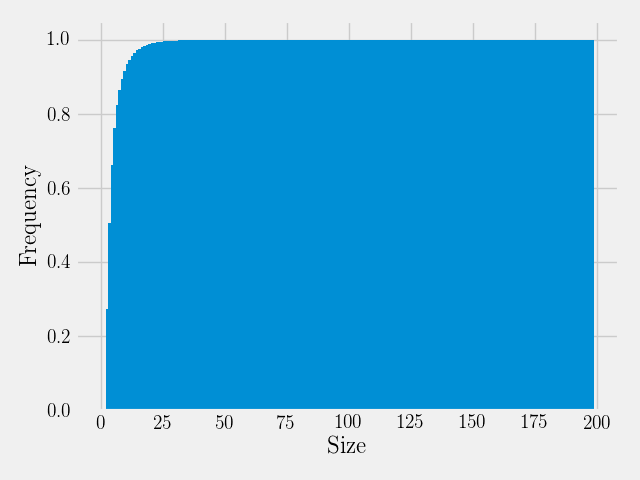
\includegraphics[width=0.3\textwidth]{intersections/total.png}
   \hfill
   \subfloat[Largest intersection including smallest iterator]{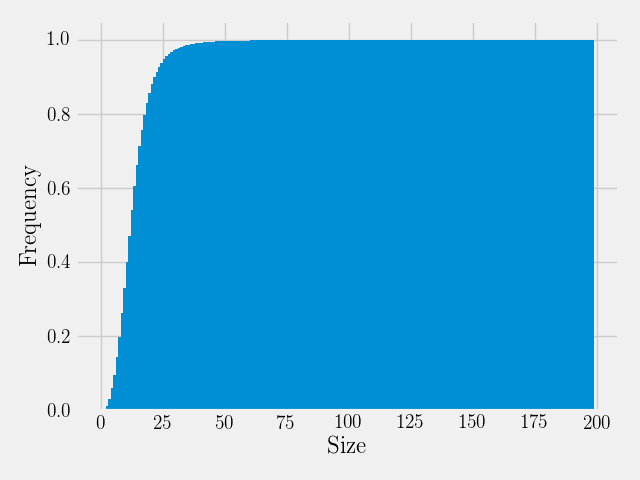
\includegraphics[width=0.3\textwidth]{intersections/smallest-biggest.png}
   \hfill
   \subfloat[Smallest iterator]{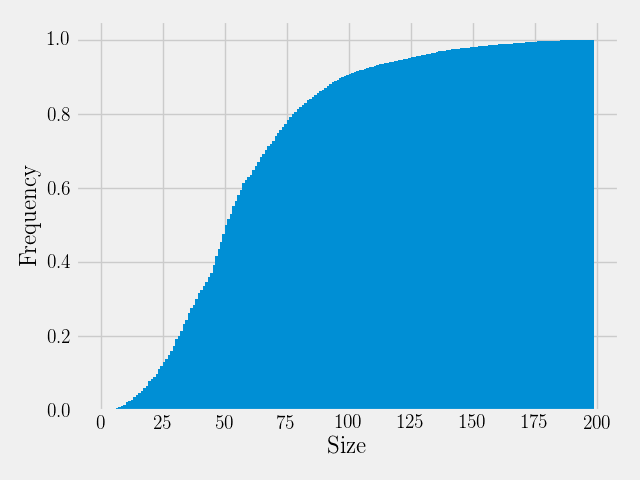
\includegraphics[width=0.3\textwidth]{intersections/smallest.png}
   \caption{Cumulative histograms of total intersection sizes, largest intersection of the smallest iterator and any other and size of the
smallest
      iterator participating in multiple queries on \texttt{SNB-sf-1}.}
   \label{fig:intersection-workload}
\end{figure}

% TODO flowy handover from paragraph to paragraph
In the coming paragraphs, we detail how to build the n-way intersection of multiple adjacency list
such that we gain performance by better use of data-locality than original the \textit{Leapfrog join}.
We choose to use pairwise intersections over multi-way intersection algorithms for their simpler,
linear memory access patterns.

From our analysis, we conclude that the final intersection size is strongly dependent on the
smallest iterator and that the intersection of the smallest iterator with any other iterator is
close to the final size.
These insight translate into two design decisions.
First, we start with the smallest iterator\footnote{We take advantage of the fact that CSR allows us
to determine the size of iterators cheaply (see~\cref{ssec:csr-impl})}.
However, we do not take the sizes of any other iterators into account because the effort for
sorting the iterators by size would not pay off.

Second, we use two different tactics to build the pairwise intersections.
The first intersection between two iterators we build by in-tandem intersection where we seek
the upper-bound of the  higher value in the smaller iterator.
This algorithm guarantees to find the intersection between two iterators in the asymtopical fastest
way.
After this first intersection, the intermediary result is quite small.
Therefore, we use the simpler scheme of linearly iterating the intermediary and probing
the iterator by binary search with fall-back to linear search.

Finally, we point out a few exceptional cases and pitfalls for implementors:
\begin{itemize}
  \item If all iterators of the \textit{Leapfrog join} are on their first level, the intersection is nearly |V|. In this case, we fall back
to the original
        \textit{Leapfrog join}.
  \item We use an array to materialize the intersections because Scala collections are slow.
        Instead of deleting elements, we replace them with a special value.
  \item Allocating a new array for every \textit{Leapfrog join} initialization is costly.
        We estimate the size of the intersection by the size of the smallest iterator and
        reuse the array whenever possible. We use a sentry element to mark the end of the array.
\end{itemize}

The carefully chosen operations explained above are faster than the original \textit{Leapfrog join}
algorithm for two reasons.
First, although, the original algorithm uses an asymtopical better n-way intersection, multiple
binary intersections are preferable with the rather small adjacency lists of graph workloads.
In particular, in our situation where the size of the first binary intersection is already
very close to the size of the final intersection.
Second, the \textit{Leapfrog join} generates a single value, then yields control to other parts
of the algorithm and later touches the same adjacency lists again to generate the next value.
Our approach touches the adjacency lists exactly once per \textit{Leapfrog} initialization and
condenses the result into a much smaller array that is more likely to stay cached while the other
parts of the join do their work.

\Cref{fig:mat-vs-nomat} shows that a materialized \textit{Leapfrog join} performance better than
the original algorithm.
As expected, the optimization is more powerful for bigger queries because they work with more
adjacency lists per \textit{Leapfrog join}, e.g. for a trianlge each \textit{Leapfrog join} intersects
only two iterators while for a \texttt{5-clique} each join handles 5 adjacency lists.
Anyhow, even for the triangle query, we see a small but clear improvement and a lower error due to
better cache use.
We refer the reader to our experiment section (\ref{sec:experiments}) for further experiments on
our graph specialized \textsc{wcoj} and detailed descriptions of the datasets and queries used.

\begin{figure}
  \centering
% TODO more queries
% TODO add amazon graph
% TODO rename dataset to materialization and no materialization or such
  \includesvg{mat-graph-bar-snb-sf1}
  \caption{Barchart showing \texttt{GraphWCOJ} with and without \textit{Leapfrog join} materialization
           enabled for different queries on \texttt{SNB-sf1}}
  \label{fig:mat-vs-nomat}
\end{figure}
